
\chapter{Calcium-induced calcium release}
\label{cicr}



We started in Chapter \ref{Ca_release_1D} by assuming that the concentrations of the junctional sarcoplasmic reticulum (JSR) and the network sarcoplasmic reticulum (NSR) are identical and that the L-type current can be ignored and thus we studied a one-dimensional problem where the calcium concentration of the dyad was the only variable of interest. The model is illustrated in Figures \ref{cicr_1D} and \ref{geom1D}. Then, in Chapter  \ref{Ca_release_2D}, we extended the model to account for the varying concentrations in the dyad and the JSR, but we still ignored the effect of the voltage-gated L-type channels and kept the concentration of the cytosol and the NSR constant. The two-dimensional model is illustrated in Figures \ref{cicr_2D} and \ref{geom2D}. Our aim is now to include the effect of L-type channels. The L-type channels open and close depending on the transmembrane potential $V$, so the model will therefore be parameterized by $V$. The model is illustrated in Figures \ref{cicr_2D_V} and \ref{geomCa_V}.

It should be noted that we are still interested in the dynamics related to the dyad and not to the whole cell. We therefore keep the concentration of the cytosol and NSR constant and assume that the concentration of the extracellular space ($c_e$) only affects the concentration of the dyad through the voltage-gated L-type calcium channels (LCCs). In a whole-cell model, this would be different in many ways, but we shall not consider that topic here.

The state of a voltage-gated channel is governed by a Markov model where the transitions depend on the transmembrane potential (or voltage for short). If the electrical potential in the dyad is given by $V_{i}$
(intracellular potential) and the extracellular potential is given by $V_{e}
$, we define the transmembrane potential to be
\[
V=V_{i}-V_{e}.
\]

As a notational convention, we use the subscript $r$ to indicate that $\bar
{\gamma}_{r}$ models the open or closed state of the ryanodine receptor (RyR)
and the subscript $l$ in the term $\bar{\gamma}_{l}J_{l}$ is used to indicate
that this is the flux through the LCC.

\begin{figure}
\centering\resizebox{0.9\linewidth}{!}{\winslow{2.5}{1.5}{8.5}{8}}
\caption{The figure is a modified version of Figure 1 (panel A) of Winslow et
al. \cite{winslow2006} and illustrates the components involved in calcium-induced calcium release (CICR). In this chapter, we concentrate on the dynamics in the box surrounded by a thin red line. We assume that the concentrations of the cytosol, the NSR, and the extracellular domain
represented by the T-tubule are kept constant and that inflow of calcium through the LCCs is governed by a voltage-dependent Markov model.
 \label{cicr_2D_V}}
\end{figure}


\newlength{\Oldarrayrulewidth}
\newcommand{\Cline}[2]{
  \noalign{\global\setlength{\Oldarrayrulewidth}{\arrayrulewidth}}
  \noalign{\global\setlength{\arrayrulewidth}{#1}}\cline{#2}
  \noalign{\global\setlength{\arrayrulewidth}{\Oldarrayrulewidth}}}


\begin{figure}
[ptb]
\begin{center}
\begin{tabular}{c!{\vrule width 1pt}c!{\vrule width 1pt}c!{\vrule width 1pt}c}
\Cline{1pt}{2-2}
&& \multicolumn{2}{c}{} \\
& Extracellular, $c_e$ & \multicolumn{2}{c}{} \\
&&  \multicolumn{2}{c}{}\\ \noalign{\hrule height 1pt}
&&& \\
Cytosol, $c_0$ & Dyad, $\bar{x}(t)$ & JSR, $\bar{y}(t)$ & NSR, $c_1$ \ \ \ \ \  \\
&&& \\ \noalign{\hrule height 1pt}
\end{tabular}
\caption{Sketch of a release unit. The cytosolic ($c_0$), NSR ($c_1$), and extracellular ($c_e$) calcium concentrations are  assumed to be constant, while the concentrations of the dyad and JSR are given by $\bar{x}=\bar{x}(t)$ and $\bar{y}=\bar{y}(t)$, respectively. Furthermore, we assume that the flux of calcium from the extracellular space to the dyad is voltage gated. Recall that $c_0\ll c_1$. }
\label{geomCa_V}
\end{center}
\end{figure}

\section[Stochastic release model parameterized by $V$]{Stochastic release model parameterized by the transmembrane potential}

\graytable{l}{
{|c|c|} \hline
$v_d $ & 1 $\rm{ms^{-1}}$\\ \hline
$v_r $ & 0.1 $\rm{ms^{-1}}$\\ \hline
$v_s $ & 0.01 $\rm{ms^{-1}}$\\ \hline
$c_0 $ & 0.1 $\rm{\mu M}$\\ \hline
$c_1 $ & 1000 $\rm{\mu M}$ \\ \hline
$c_e $ & 1800 $\rm{\mu M}$ \\ \hline
}{Values of parameters used in simulations in this chapter.
%${\ }^*$Unless otherwise stated.
\label{tab:param2DV}}



%}{Values of parameters used in 2D simulations based on the scheme (\ref{nc1},\ref{nc2}). \label{tab:param2D}}

In the models we have studied so far, a very basic building block has been
that, if $x_{0}$ denotes the concentration of a large reservoir of calcium and
$x=x(t)$ denotes the concentration of a small space connected to the reservoir,
then the concentration $x$ evolves according to the model
\begin{equation}
x^{\prime}(t)=v\left(  x_{0}-x(t)\right),  \label{linflux}
\end{equation}
where $v$ denotes the speed of diffusion between the two spaces. Here we assume that the concentration of the large reservoir, $x_0$, can be kept constant.  This model
can be extended to the case where the channel between the spaces can be either
closed or open:
\begin{equation}
\bar{x}^{\prime}(t)=\bar{\gamma}(t)v\left(  x_{0}-\bar{x}(t)\right),
\label{s_linfux}
\end{equation}
where $\bar{\gamma}$ is a random variable taking on two possible values, one
(open) and zero (closed). The stochastic release models studied above are derived by
gluing together pieces of models of exactly this type.

 In this chapter, one
additional effect is added: We now allow calcium to flow into the dyad
through the LCCs. This flow depends on both the
gradient of the concentration and of the electrical potential across the membrane
dividing the extracellular space and the dyad.

The process illustrated in Figure \ref{geomCa_V} can be modeled as follows
\begin{align}
\bar{x}^{\prime} &  =\bar{\gamma}_{r}v_{r}\left(  \bar{y}-\bar{x}\right)
+v_{d}\left(  c_{0}-\bar{x}\right)  -\bar{\gamma}_{l}J_{l},\label{c1v}\\
\bar{y}^{\prime} &  =\bar{\gamma}_{r}v_{r}\left(  \bar{x}-\bar{y}\right)
+v_{s}\left(  c_{1}-\bar{y}\right)  .\label{c2v}
\end{align}
This model is almost the same as the one we analyzed above (see  $(
\ref{c1})$ and $(\ref{c2})  $ on page \pageref{c1}). The new term is given by
$-\bar{\gamma}_{l}J_{l}$ and it models the inflow of calcium through the
LCCs. The function $\bar{\gamma}_{l}$ is governed by a Markov model and, as
usual, it takes on two values: zero (closed) and one (open). The Markov model
governing $\bar{\gamma}_{l}$ depends on the transmembrane potential $V$ and
the flux depends on $V,$ the extracellular calcium concentration $c_{e}$ and the dyad concentration $x=x(t).$ As above, $v_{r}$ denotes the rate of release
from the JSR to the dyad, $v_{d}$ denotes the speed of calcium diffusion from the dyad
to the cytosol, and $v_{s}$ denotes the speed of calcium diffusion from the NSR
 to the JSR.

The Markov model governing $\bar{\gamma}_{r}$ will be the same as above, but we need to
introduce a Markov model governing $\bar{\gamma}_{l}$. We will also combine these Markov models
to simplify the introduction of a probability density formulation. Furthermore, we need to describe the electrochemical flux $J_{l}$.

\subsection{Electrochemical Goldman--Hodgkin--Katz (GHK) flux}

Consider Figure \ref{cicr_2D_V} and suppose that the membrane between the
T-tubule and the dyad has thickness $L.$ If the electrical field is
constant through the channel, the flux is given by
\begin{equation}
J_{l}=\frac{D}{L}\frac{2F}{RT}\frac{x-c_{e}e^{-\frac{2FV}{RT}}}{1-e^{-\frac
{2FV}{RT}}}V, \label{GHK}
\end{equation}
\graytable{l}{
{|c|c|} \hline
$F$ & $96485.3$ C mol$^{-1}$\\ \hline
$R$ & $8.3145$ J mol$^{-1}$K$^{-1}$\\\hline
$T$ & 310 K\\\hline
$V_0$ & 13.357 mV\\ \hline
$\frac{D}{L}$&0.02 ms$^{-1}$\\ \hline
}{Parameters in (\ref{GHK}).\label{FRT}}
which is referred to as the GHK flux (see Keener and Sneyd \cite{KeenerSneyd}). Here $D$ is
Fick's diffusion constant, $F$ is Faraday's constant, $R$ is the gas constant,
and $T$ is the absolute temperature.
By defining
\[
V_0=\frac{RT}{2F},
\]
we have
\begin{equation}
J_{l}=\frac{D}{L}\frac{x-c_{e}e^{-\frac{V}{V_0}}}{1-e^{-\frac{V}{V_0}}}\frac{V}{V_0},\label{fluxJ}
\end{equation}
where $F,R,T$, and $V_0$ are given in Table \ref{FRT}.
%\[
%\begin{tabular}
%[c]{ll}
%$F$ & $96485.3$ C mol$^{-1}$\\
%$R$ & $8.3145$ J mol$^{-1}$K$^{-1}$\\
%$T$ & 310 K\\
%$V_0$ & 13.357 mV\\[1mm]
%$\frac{D}{L}$&0.02ms$^{-1}$
%\label{FRT}
%\end{tabular}
%\]

%\K{zzz Jeg pr\o ver \r{a} se p\r{a} enhetene her.
%Hva er enhetene til D og L? Hvis det er $\text{dm}^{2}/(\text{ms})$
%og dm, f\r{a}r vel $J_l$ enhet $\mu \text{mol}/(\text{ms dm}^2)$ mens de andre leddene i
%(8.3) og (8.4) har enhet $\mu \text{mol}/(\text{ms dm}^3)$?
%Men slik er det vel ikke? }
%\G{We only need to know the ratio, we have used $D/L = v_l = 0.02$/ms. The symbol $v_l$ is not used in the text, but perhaps it should.}

\subsection{Assumptions}

As for the model in Chapter  \ref{Ca_release_2D}, we will make the following assumptions for the parameters involved:
\begin{align}
 c_{1}&\gg c_{0} \, \mbox{ and } \, v_r,v_d,v_s >0,  \label{assumption1V} \\
 v_{d}v_{s}&\ge v_{r}^{2}.  \label{assumption2V}
\end{align}

\begin{comment}
In the present model the transmembrane potential is a parameter and we will assume that it satisfies the condition
\begin{equation}
V\leqslant V_{0}\ln\left(  \frac{v_{r}+v_{d}}{c_{1}v_{r}+c_{0}v_{d}}
c_{e}\right). \label{cond_V_200}
\end{equation}
With the parameters used in our computations (see Table \ref{tab:param2DV}),  this condition implies
that we consider transmembrane potentials satisfying the condition
\begin{equation}
V\leqslant39.87\text{mV.}\label{cond_V_201}
\end{equation}
\end{comment}


\subsection{Equilibrium potential}

\bigskip The electrochemical equilibrium over the membrane separating the
extracellular space and the dyad is characterized by
\[
J_{l}=0.
\]
In equilibrium, we must have
\[
x=c_{e}e^{-\frac{V}{V_0}},
\]
so the equilibrium transmembrane potential is given by
\begin{equation}
V_{eq}=V_0 \ln\frac{c_{e}}{x}\label{V_eq}.
\end{equation}
For this value of the transmembrane potential $V,$ the driving force $\, -\bar{\gamma}_{l}J_{l}$ in the
system (\ref{c1v}) and (\ref{c2v}) is zero even if the channel is open. It
should also be noted that the equilibrium transmembrane potential depends on
the concentration $x$ of the dyad and will therefore be a dynamic quantity. Here it is useful to
recall that we regard $V$ as a parameter input to the system and not a part of the dynamics.

\bigskip

\subsection{Linear version of the flux}

We mentioned above that our modeling so far has been based on very simple
linear fluxes of the form given in (ref{linflux}) In the
case we are considering now, the flux depends on both the difference in
concentration and the electrical potential over the membrane; see $\left(
\ref{fluxJ}\right)$.  A Taylor series expansion of the GHK flux can be written as

\begin{equation}
J_{l}=\allowbreak\frac{D}{L}\left(  x-c_{e}\right)  +\frac{D}{2L}\left(
x+c_{e}\right)  \frac{V}{V_0} +O\left( \left( V\slash V_0\right)^{2}\right) \label{l_flux}
\end{equation}
and, therefore, if $V=0,$ the flux is given by
\[
J_{l}=\frac{D}{L}\left(
x-c_{e}\right)
\]
so the term $-\bar{\gamma}_{l}J_{l} $ has the form we used
in (ref{s_linfux}) This means that the electrochemical flux given by $\left(
\ref{fluxJ}\right)$ reduces to a purely concentration-based flux
 when there is no difference in electrical potential across the membrane.

%\K{zzz Jeg klarer ikke \r{a} utlede denne Taylor-utviklingen. Skal det egentlig
%v\ae re $O(( \frac{V}{V_0})^{2})$ eller spiller ikke det noen rolle?}

\subsection{Markov models for CICR}

As discussed above, two Markov processes are involved in the CICR. We have seen that the gating of the release of
calcium from the sarcoplasmic reticulum to the dyad is given by the stochastic variable
$\bar{\gamma}_{r}=\bar{\gamma}_{r}(t)$, which is governed by the reaction
scheme
\begin{equation}
C_{r}\underset{k_{co}^{r}}{\overset{k_{oc}^{r}}{\leftrightarrows}}O_{r}.
\label{m_r}
\end{equation}
We recall here that $r$ is used to indicate the relation to the RyR
channels. Similarly, the Markov model for the LCC is given by
\begin{equation}
C_{l}\underset{k_{co}^{l}}{\overset{k_{oc}^{l}}{\leftrightarrows}}O_{l},
\label{m_l}
\end{equation}
where $l$ is used to indicate the relation to the LCCs.
This Markov model governs the stochastic variable $\bar{\gamma}_{l}
=\bar{\gamma}_{l}(t).$

It is convenient to combine these two Markov models into one reaction scheme
of the form illustrated in Figure \ref{eq:m_rl}.
\begin{figure}[ptb]
\begin{center}
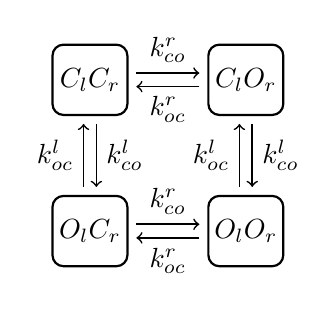
\begin{tikzpicture}[
   font=\sffamily,
   every matrix/.style={ampersand replacement=\&,column sep=1cm,row sep=1cm},
   state/.style={draw,thick,rounded corners,inner sep=.3cm},
   to/.style={->,semithick,shorten >=0.1cm,shorten <=0.1cm},
   Q/.style={->,semithick,sloped,pos=0.700000,shorten >=0.1cm,shorten <=0.1cm},
   every node/.style={auto}]
\matrix{
\node[state] (C_{l}C_{r}) {\parbox{10pt}{\centerline{$C_{l}C_{r}$}}};\&\node[state] (C_{l}O_{r}) {\parbox{10pt}{\centerline{$C_{l}O_{r}$}}};\\
\node[state] (O_{l}C_{r}) {\parbox{10pt}{\centerline{$O_{l}C_{r}$}}};\&\node[state] (O_{l}O_{r}) {\parbox{10pt}{\centerline{$O_{l}O_{r}$}}};\\
};
\draw[to]  (C_{l}C_{r}.10) to node {$k_{co}^{r}$} (C_{l}O_{r}.170);
\draw[to]  (C_{l}C_{r}.280) to node {$k_{co}^{l}$} (O_{l}C_{r}.80);
\draw[to]  (C_{l}O_{r}.190) to node {$k_{oc}^{r}$} (C_{l}C_{r}.350);
\draw[to]  (C_{l}O_{r}.280) to node {$k_{co}^{l}$} (O_{l}O_{r}.80);
\draw[to]  (O_{l}C_{r}.100) to node {$k_{oc}^{l}$} (C_{l}C_{r}.260);
\draw[to]  (O_{l}C_{r}.10) to node {$k_{co}^{r}$} (O_{l}O_{r}.170);
\draw[to]  (O_{l}O_{r}.100) to node {$k_{oc}^{l}$} (C_{l}O_{r}.260);
\draw[to]  (O_{l}O_{r}.190) to node {$k_{oc}^{r}$} (O_{l}C_{r}.350);
\end{tikzpicture}
\end{center}
\caption{Markov model including four possible states: $C_{l}C_{r}$ (both
closed), $C_{l}O_{r}$ (LCC closed, RyR open), $O_{l}O_{r}$ (both open), and
$O_{l}C_{r}$ (LCC open, RyR closed).}
\label{eq:m_rl}
\end{figure}
The states of this combined Markov model are given by $C_{l}C_{r}$ (both
closed), $C_{l}O_{r}$ (LCC closed, RyR open), $O_{l}O_{r}$ (both open), and
$O_{l}C_{r}$ (LCC open, RyR closed). In our computations, we use the rates shown in Table \ref{tab:rate}.
%following functions
%\begin{equation}
\begin{table}
\begin{center}
%\begin{tabular}[c]{|l|l|l|l|} \hline
%$k_{co}^{r}=\mu \frac{x^4}{K(y)^4+x^4}$ & $k_{oc}^{r}=1$ &
%$K(y) =  K_{max}-y/1000$ & $K_{max} = 7.4\mu$M \\ \hline
%$k_{co}^{l}=\eta\, l_{\infty}(V)/\tau_l$ & $k_{oc}^{l}=(1-l_{\infty}(V))/\tau_l%$ &$l_{\infty}(V) = 0.01 \exp(-(V-5)^2/500)$
%&$\tau_l=1$ms \\ \hline
\begin{tabular}[c]{|l|l|} \hline
RyR: & LCC: \\
$k_{co}^{r}=\mu \frac{x^4}{K(y)^4+x^4} \text{ ms}^{-1}$ &$k_{co}^{l}=\eta\, l_{\infty}(V)/\tau_l$ \\
$k_{oc}^{r}=1 \text{ ms}^{-1}$ & $k_{oc}^{l}=(1-l_{\infty}(V))/\tau_l$ \\
$K(y) =  K_{max}-y/1000$ &  $l_{\infty}(V) = 0.01 \exp(-(V-5)^{2}/500)$ \\
$K_{max} = 7.4$ $\mu$M & $\tau_l=1$ ms\\ \hline
\end{tabular}
\end{center}
%\end{equation}
\caption{Reaction rates used in the Markov model illustrated in
Figure \ref{eq:m_rl}.
 Here $\mu \ge 1$ denotes the mutation severity
index of the RyR, $\eta \ge 1$ denotes the mutation severity
index of the LCC and $\mu=\nu=1$ represents the wild type case.
\label{functions}
\label{tab:rate}}
\end{table}

\subsection{Numerical scheme for the stochastic CICR  model}

 A numerical scheme for running simulations based on the CICR model
($\ref{c1v}$) and ($\ref{c2v}$)
is given by
\begin{align}
x_{n+1} &  =x_{n}+\Delta t\left(  \gamma_{n}^{r}v_{r}\left(  y_{n}
-x_{n}\right)  +v_{d}\left(  c_{0}-x_{n}\right)  \right)  -\Delta t \gamma_{n}^{l}
J_{l}(x_{n},V),\label{nc1v}\\
y_{n+1} &  =y_{n}+\Delta t\left(  \gamma_{n}^{r}v_{r}\left(  x_{n}
-y_{n}\right)  +v_{s}\left(  c_{1}-y_{n}\right)  \right)  ,\label{nc2v}
\end{align}
where $\gamma_{n}^{r}$ and $\gamma_{n}^{l}$ are computed according to the
Markov model illustrated in Figure \ref{eq:m_rl}.

\subsection{Monte Carlo simulations of CICR}

In Figure \ref{cicr:cicr}, we show the results of stochastic simulations
using the model $(\ref{c1v})$ and $(\ref{c2v}) $.
The computations are based on the numerical scheme
$(\ref{nc1v})$  and $(\ref{nc2v}) $ with the parameters given in Table \ref{tab:param2DV} and $\Delta t=0.01$ ms. As initial conditions we have used $x(0) = c_0$ and $y(0) = c_1$ with both gates closed.
From top to bottom, the transmembrane potential is given by $V=20$ mV, $0$ mV, $-20$ mV, and $-40$ mV.

The associated calcium concentrations of the dyad given by $x=x(t)$ are graphed in the left panels and the
calcium concentrations of the JSR given by $y=y(t)$ are graphed in the right panels.
In all cases, we show the solution for a time interval ranging from 0 ms to 1000 ms.
The calcium concentration clearly depends on the transmembrane potential and we observe in particular that there
is no activity for $V=-40$ mV, since the LCC is inactivated at that voltage.

In Figure \ref{cicr:zoom}, we show a detailed view of the case of $V=0$ mV.
In the upper part of the graph we show the state
of the RyR (upper) and the LCCs (lower). The CICR mechanism is illustrated in the first part of the graph: The LCC opens at $t \approx 5$ ms, but the release is too short-lived to trigger an RyR opening and we therefore observe just a minor increase in the dyad calcium concentration given by  $x$. Next time, at
$t \approx 9$ ms, there is a new opening and now the channel is open for a longer time;
there is an increase in $x$ leading to opening of the RyR channel and then the concentration increases dramatically.

FIGURE: [fig/cicr_cicr.pdf, width=500 frac=0.8] Calcium dynamics of the dyad $x=x(t)$ and the JSR $y=y(t)$ for four values of the transmembrane potential $V$. labe{circ:circ}

FIGURE: [fig/cicr_zoom.pdf, width=500 frac=0.8] A detailed view of the case of $V=0$ mV taken from Figure \ref{cicr:cicr}. In addition, we show the state of the RyR channel (upper panel) and the LCC (lower panel). The first spike at 5 ms in the LCC is very short and does not trigger an RyR release. The next one, at 9 ms, does trigger an RyR release. label{cicr:zoom}

\section{Invariant region for the CICR model}

We have seen in both the one- and two-dimensional models above that we can derive invariant
regions for the stochastic models and that these regions define the
computational domain for the probability density system. Our aim is now to
derive an invariant region for the CICR model given by
\begin{align}
\bar{x}^{\prime}  &  =\bar{\gamma}_{r}v_{r}\left(  \bar{y}-\bar{x}\right)
+v_{d}\left(  c_{0}-\bar{x}\right)  -\bar{\gamma}_{l}J_{l},\label{c1v2}\\
\bar{y}^{\prime}  &  =\bar{\gamma}_{r}v_{r}\left(  \bar{x}-\bar{y}\right)
+v_{s}\left(  c_{1}-\bar{y}\right)  . \label{c2v2}
\end{align}
Here it is convenient to write the GHK flux in the form
\[
J_{l}(x)=a_{0}(x-x_{0}),
\]
where
\[
a_{0}=\frac{D}{L}\frac{1}{1-e^{-\frac{V}{V_{0}}}}\frac{V}{V_{0}}
\]
and
\[
x_{0}=c_{e}e^{-\frac{V}{V_{0}}},
\]
so the system takes the form
\begin{align}
\bar{x}^{\prime}  &  =\bar{\gamma}_{r}v_{r}\left(  \bar{y}-\bar{x}\right)
+v_{d}\left(  c_{0}-\bar{x}\right)  +\bar{\gamma}_{l}a_{0}(x_{0}-\bar
{x}),\label{xc1v2}\\
\bar{y}^{\prime}  &  =\bar{\gamma}_{r}v_{r}\left(  \bar{x}-\bar{y}\right)
+v_{s}\left(  c_{1}-\bar{y}\right)  . \label{yc2v2}
\end{align}


\subsection{A numerical scheme}

Let us consider the numerical scheme (\ref{nc1v}, \ref{nc2v}),
\begin{align}
x_{n+1}  &  =x_n+\Delta t\left( \gamma_n^{r}v_{r}\left(  y-x\right)  +v_{d}\left(
c_{0}-x\right)  +\gamma_n^{l}a_{0}(x_{0}-x)\right) ,\label{x400}\\
y_{n+1} &  =y_n+\Delta t\left(\gamma_n^{r}v_{r}\left(  x-y\right)  +v_{s}\left(
c_{1}-y\right) \right)  . \label{y400}
\end{align}
Here $\gamma_n^{r}$ and $\gamma_n^{l}$ simply denotes constants that take on the
value zero or one and their values will be specified in order to study the
dynamics of the system when the associated channels are open or closed. The
numerical scheme can be written in the form
\begin{align}
x_{n+1} &  =F\left(  x_{n},y_{n}\right)  ,\label{x401}\\
y_{n+1} &  =G\left(  x_{n},y_{n}\right)  ,\label{y401}
\end{align}
with
\begin{align*}
F(x,y) &  =x+\Delta t\left(  \gamma_{r}v_{r}\left(  y-x\right)  +v_{d}\left(
c_{0}-x\right)  +\gamma_{l}a_{0}(x_{0}-x)\right)  ,\\
G(x,y) &  =y+\Delta t\left(  \gamma_{r}v_{r}\left(  x-y\right)  +v_{s}\left(
c_{1}-y\right)  \right).
\end{align*}
Here we assume that
\begin{equation}
\Delta t\leqslant\min\left(  \frac{1}{v_{d}+a_{0}+v_{r}},\frac{1}{v_{s}+v_{r}
}\right).  \label{dt400}
\end{equation}
Under this condition, we observe that
\[
\frac{\partial F}{\partial x}=1-\Delta t\left(  v_{d}+\gamma_{l}a_{0}
+\gamma_{r}v_{r}\right)  \geqslant0
\]
for any choice of $\gamma_{l}$ and $\gamma_{r}$. We also have
\[
\frac{\partial F}{\partial y}=\Delta t \gamma_{r}v_{r}\geqslant0.
\]
Similarly, we find that
\begin{equation}
\frac{\partial G}{\partial x}=\Delta t \gamma_{r}v_{r}\geqslant0
\end{equation}
and
\begin{equation}
\frac{\partial G}{\partial y}=1-\Delta t\left(  v_{s}+\gamma_{r}v_{r}\right)
\geqslant0.
\end{equation}
Assume that
\begin{equation}
0\leqslant x_{n},y_{n}\leqslant M,\label{y411}
\end{equation}
where
\[
M=\max\left(  c_{1},\frac{c_0 v_d +a_{0}x_{0}}{a_{0}+v_{d}}\right)  .
\]
Since
\[
\frac{\partial F}{\partial x},\frac{\partial F}{\partial y},\frac{\partial
G}{\partial x},\frac{\partial G}{\partial y}\geqslant0,
\]
we have
\[
x_{n+1}=F\left(  x_{n},y_{n}\right)  \leqslant F(M,M)=M+\Delta t\left(
v_{d}\left(  c_{0}-M\right)  +\gamma_{l}a_{0}(x_{0}-M)\right)  \leqslant M
\]
and
\[
y_{n+1}=G\left(  x_{n},y_{n}\right)  \leqslant G(M,M)=M+\Delta t\left(
v_{s}\left(  c_{1}-M\right)  \right)  \leqslant M.
\]
Furthermore, we have
\[
x_{n+1}=F\left(  x_{n},y_{n}\right)  \geqslant F(0,0)=\Delta t\left(
v_{d}c_{0}+\gamma_{l}a_{0}x_{0}\right)  \geqslant0
\]
and
\[
y_{n+1}=G\left(  x_{n},y_{n}\right)  \geqslant G(0,0)=\Delta tv_{s}
c_{1}\geqslant0.
\]
So, by induction, the invariant region (ref{y411}) holds for
all $n\geqslant0.$


\section[Probability density model parameterized by V]{Probability density model parameterized by the transmembrane potential}


The probability density formulation of the system ($\ref{c1v}$) and ($\ref{c2v}$) is given by the
 system of partial differential equations
\begin{align}
\frac{\partial\rho_{oo}}{\partial t}+\frac{\partial}{\partial x}\left(
a_{oo}^{x}\rho_{oo}\right)  +\frac{\partial}{\partial y}\left(  a_{oo}^{y}
\rho_{oo}\right)   &  =k_{co}^{l}\rho_{co}-\left(  k_{oc}^{l}+k_{oc}
^{r}\right)  \rho_{oo}+k_{co}^{r}\rho_{oc},\label{eq:pdfoo}\\
\frac{\partial\rho_{oc}}{\partial t}+\frac{\partial}{\partial x}\left(
a_{oc}^{x}\rho_{oc}\right)  +\frac{\partial}{\partial y}\left(  a_{oc}^{y}
\rho_{oc}\right)   &  =k_{co}^{l}\rho_{cc}-\left(  k_{oc}^{l}+k_{co}
^{r}\right)  \rho_{oc}+k_{oc}^{r}\rho_{oo},\label{eq:pdfoc}\\
\frac{\partial\rho_{cc}}{\partial t}+\frac{\partial}{\partial x}\left(
a_{cc}^{x}\rho_{cc}\right)  +\frac{\partial}{\partial y}\left(  a_{cc}^{y}
\rho_{cc}\right)   &  =k_{oc}^{l}\rho_{oc}-\left(  k_{co}^{l}+k_{co}
^{r}\right)  \rho_{cc}+k_{oc}^{r}\rho_{co},\label{eq:pdfcc}\\
\frac{\partial\rho_{co}}{\partial t}+\frac{\partial}{\partial x}\left(
a_{co}^{x}\rho_{co}\right)  +\frac{\partial}{\partial y}\left(  a_{co}^{y}
\rho_{co}\right)   &  =k_{oc}^{l}\rho_{oo}-\left(  k_{co}^{l}+k_{oc}
^{r}\right)  \rho_{oc}+k_{co}^{r}\rho_{cc},\label{eq:pdfco}
\end{align}
where $\rho_{oo},\rho_{oc},\rho_{cc},$ and $\rho_{co}$ represent the probability
densities of the states denoted
$O_{l}O_{r},O_{l}C_{r},C_{l}C_{r},$ and $C_{l}O_{r},$ respectively. The terms of the fluxes are given by
\[
\begin{tabular}
[c]{ll}
$a_{oo}^{x}=v_{r}\left(  y-x\right)  +v_{d}\left(  c_{0}-x\right)
-J_{l}(x,V),$ & $a_{oo}^{y}=v_{r}\left(  x-y\right)  +v_{s}\left(
c_{1}-y\right),  $\\
$a_{oc}^{x}=v_{d}\left(  c_{0}-x\right) - J_{l}(x,V),$ &
$a_{oc}^{y}=v_{s}\left(  c_{1}-y\right),  $\\
$a_{cc}^{x}=v_{d}\left(  c_{0}-x\right),  $ & $a_{cc}^{y}=v_{s}\left(
c_{1}-y\right),  $\\
$a_{co}^{x}=v_{r}\left(  y-x\right)+v_{d}\left(  c_{0}-x\right),  $ & $a_{co}^{y}
=v_{r}\left(  x-y\right)  +v_{s}\left(  c_{1}-y\right),  $
\end{tabular}
\]
where we use the convention that in the expression $a_{\alpha\beta}
^{x},$ the index $\alpha$ indicates whether the LCC is open
$(\alpha=o)$ or closed $(\alpha=c)$ and the index $\beta$ plays the same role
for the RyR channel. Similar notation is used for the flux terms represented by
$a_{\alpha\beta}^{y}.$ As usual, the sum of total probabilities is
one:
\begin{equation}
\int_{\Omega}\left(  \rho_{oo}+\rho_{oc}+\rho_{cc}+\rho_{co}\right)  dx\,dy=1. \label{sumone}
\end{equation}



\section{Computing probability density representations of CICR}

 In Figure \ref{cicr:Vdep}, we show solutions of the system ($\ref{c1v2}$) and ($\ref{c2v2}$) defined in the computational domain
 $\Omega=\Omega(V)$ for four values of the transmembrane potential: $V = 20$ mV, $0$ mV, $-20$ mV, and $-40$ mV. In all computations, the parameters are given in Table \ref{tab:param2DV} and the Markov model is illustrated in Figure \ref{eq:m_rl}.
All distributions are initially set to zero, except that $\rho_{cc}(c_0,c_1)= 1/(\Delta x \Delta y)$. Hence the initial discrete probability densities integrates to one;
\begin{equation}
\Delta x \Delta y \sum_{i,j}  \rho_{i,j}=1,  % \label{discrete_sumone}
\end{equation}
which is a discrete version of $(\ref{sumone})$ with $\rho=\rho_{oo}+\rho_{oc}+\rho_{co}+\rho_{cc}$.

The simulation results are shown in Figure \ref{cicr:Vdep}  and summarized in Table \ref{tab:stat2DV}. We observe that the transmembrane potential $V$ significantly influences the probability density functions. In Table \ref{tab:stat2DV}, we observe that the probability of the LCC being in the open state is highest for $V=0$ mV and it is almost zero for $V=-40$ mV. In the computations, we use $\Delta t=0.001$ ms, $\Delta x=1.02$ $\mu$M, $1.23$ $\mu$M, $1.54$ $\mu$M and $1.95$ $\mu$M (the domain size varies with $V$), and $\Delta y=9.3$ $\mu$M. Note that the scale of the plots varies (see Figure \ref{cicr:Vdep}).


FIGURE: [fig/cicr_Vdep.pdf, width=500 frac=0.8] Probability density functions for different voltages. The LCC is more prone to being open (last two columns) when the voltage is close to $V=5$ mV, that is, where $l_{\infty}(V)$ is close to its maximum. Black corresponds to $10^{-3}$ for $\rho_{cc}$ and to $10^{-6}$ for the other three distributions. label{cicr:Vdep}

\begin{table}  \begin{center}
\begin{tabular}{|r|r|r|r|r|} \hline
 $V$ & $\pi_{cc}$ & $\pi_{co}$ & $\pi_{oc}$ & $\pi_{oo}$ \\ \hline
20 & 0.978 & 0.015 & 0.005 & 0.001 \\ \hline
0 & 0.959 & 0.032 & 0.007 & 0.003 \\ \hline
-20 & 0.982 & 0.015 & 0.002 & 0.001 \\ \hline
-40 & 0.993 & 0.006 & 0.000 & 0.000 \\ \hline
\end{tabular} \end{center}
\caption{Probability of being in the four states for different voltages. Recall that the probabilities are computed
using  (\ref{probability}) at page \pageref{probability} where the probability density functions are numerical solutions
of the system (\ref{eq:pdfoo})-(\ref{eq:pdfco}).}
\label{tab:stat2DV}
\end{table}




\section{Effects of LCC and RyR mutations}

We are now in a position to study the effect of both LCC and RyR
mutations. We assume that both the LCC and RyR mutations lead to leaky
channels that can be represented by increasing the reaction rate from
closed to open. So we again consider CO-mutations.

The reaction scheme in the presence of mutations is illustrated in Figure \ref{Eq:m_rl_m}.
Here $\mu\geq1$ denotes the
strength of the RyR mutations and $\eta\geq1$ denotes the strength of the LCC
mutations. Note that $\mu=1$ and $\eta=1$ represent the wild type.

\begin{figure}[ptb]
\begin{center}
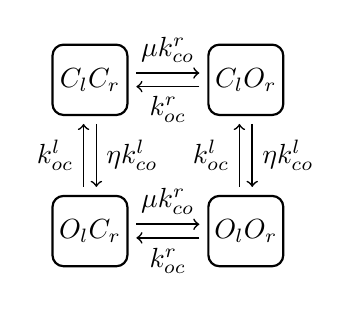
\begin{tikzpicture}[
   font=\sffamily,
   every matrix/.style={ampersand replacement=\&,column sep=1cm,row sep=1cm},
   state/.style={draw,thick,rounded corners,inner sep=.3cm},
   to/.style={->,semithick,shorten >=0.1cm,shorten <=0.1cm},
   Q/.style={->,semithick,sloped,pos=0.700000,shorten >=0.1cm,shorten <=0.1cm},
   every node/.style={auto}]
\matrix{
\node[state] (C_{l}C_{r}) {\parbox{10pt}{\centerline{$C_{l}C_{r}$}}};\&\node[state] (C_{l}O_{r}) {\parbox{10pt}{\centerline{$C_{l}O_{r}$}}};\\
\node[state] (O_{l}C_{r}) {\parbox{10pt}{\centerline{$O_{l}C_{r}$}}};\&\node[state] (O_{l}O_{r}) {\parbox{10pt}{\centerline{$O_{l}O_{r}$}}};\\
};
\draw[to]  (C_{l}C_{r}.10) to node {$\mu k_{co}^{r}$} (C_{l}O_{r}.170);
\draw[to]  (C_{l}C_{r}.280) to node {$\eta k_{co}^{l}$} (O_{l}C_{r}.80);
\draw[to]  (C_{l}O_{r}.190) to node {$k_{oc}^{r}$} (C_{l}C_{r}.350);
\draw[to]  (C_{l}O_{r}.280) to node {$\eta k_{co}^{l}$} (O_{l}O_{r}.80);
\draw[to]  (O_{l}C_{r}.100) to node {$k_{oc}^{l}$} (C_{l}C_{r}.260);
\draw[to]  (O_{l}C_{r}.10) to node {$\mu k_{co}^{r}$} (O_{l}O_{r}.170);
\draw[to]  (O_{l}O_{r}.100) to node {$k_{oc}^{l}$} (C_{l}O_{r}.260);
\draw[to]  (O_{l}O_{r}.190) to node {$k_{oc}^{r}$} (O_{l}C_{r}.350);
\end{tikzpicture}
\end{center}
\caption{Mutant version of the Markov model given in Figure \ref{eq:m_rl}
including four possible states: $C_{l}C_{r}$ (both
closed), $C_{l}O_{r}$ (LCC closed, RyR open), $O_{l}O_{r}$ (both open), and
$O_{l}C_{r}$ (LCC open, RyR closed).}
\label{Eq:m_rl_m}
\end{figure}



\subsection{Effect of mutations measured in a norm}

To
measure the effect of the mutations, we introduce the norm
\begin{equation}
\Vert \rho^{\eta,\mu}-\rho^{1,1}\Vert=\frac{1}{6}\sum_{V} \sum_{z}\frac{\Vert\rho_z^{\eta,\mu}-\rho_z^{1,1}\Vert_{L^{2}\left(  \Omega\right)  }}{\Vert\rho_z^{\eta,\mu}\Vert_{L^{2}\left(  \Omega\right)}+\Vert\rho_z^{1,1}\Vert_{L^{2}\left(  \Omega\right)}, \label{norm44}}
\end{equation}
where $\rho_z$ represents $\rho_{oo}$,$\, \rho_{oc}$,$\, \rho_{co}$, or
$\rho_{cc}$ and $V$ represents summation over the following values of the transmembrane potential: $-80$ mV, $-60$ mV, $-40$ mV, $-20$ mV, $0$ mV, and $20$ mV. Furthermore,
\begin{equation}
\Vert\rho\Vert_{L^{2}\left(  \Omega\right)  }=\left(\int_{\Omega}\rho^2 d\Omega\right) ^{1/2}. \label{norm_rho}
\end{equation}


The difference between the wild type solution and the solution based on
mutated reaction rates is depicted in Figure \ref{cicr:mutations}.
The figure shows the difference as a function of the two mutation severity indices $\mu$ and $\eta$.


FIGURE: [fig/cicr_mutations.pdf, width=500 frac=0.8] Difference between wild type solutions and mutated solutions, defined in terms of the norm given by (\ref{norm44}). The wild type solution is represented by $\mu=\eta=1$. label{cicr:mutations}

\subsection{Mutations increase the open probability of both the LCC and RyR channels}

In Section \ref{statistics} (page \pageref{statistics}), we introduced statistical measures for the probability density functions. We will now consider how the LCC and RyR mutations affect the statistical properties of the associated probability density functions. Let us first consider how the mutations affect the total probability of being in the different states. In Figure \ref{cicr:mut_I}, we show the total probability of being in the states OO, CO, OC, and CC, where, as above, the first letter denotes the state of the LCC and the second letter indicates the state of the RyR channel. Here the value of the transmembrane potential is $V=0$ mV.
In  Figure \ref{cicr:mut_IV80}, we show similar results in the case of $V=-80$ mV; the probability of the LCC being open is very small and the LCC mutation must be extremely severe to change this. Basically, at $V=-80$ mV, the LCC is closed independent of the mutations. This observation certainly depends heavily on the particular reaction rates used in these computations (see Table (\ref{functions}) on page \pageref{functions}).



FIGURE: [fig/cicr_mut_I.pdf, width=500 frac=0.8] Probability of being in the state OO, CO, OC, or CC at $V=0$ mV as a function of the mutation severity index of the LCC, represented by $\eta$, and the mutation severity index of the RyR channel, represented by $\mu$. Here $\eta=\mu=1$ represents the wild type. label{cicr:mut_I}

FIGURE: [fig/cicr_mut_IV80.pdf, width=500 frac=0.8] Probability of being in the state OO, CO, OC, or CC at $V=-80$ mV as a function of the mutation severity index of the LCC, represented by $\eta$, and the mutation severity index of the RyR channel, represented by $\mu$. Here $\eta=\mu=1$ represents the wild type. Note the scale of the axis in the plots on the left-hand side. label{cicr:mut_I}


\subsection{Mutations change the expected values of concentrations}

 Figures \ref{cicr:mut_XY} and \ref{cicr:mut_XYV80} show the development of the expected concentration for varying strengths of mutations. In Figure \ref{cicr:mut_XY}, we set $V=0$ mV and see that the mutations change the expected concentrations significantly. More specifically, both mutations lead to lower expected JSR concentrations. In Figure \ref{cicr:mut_XYV80}, we set $V=-80$ mV and observe that the expected concentrations are not altered by the LCC mutation. As for the total probabilities discussed above, the reason for this is that, at this value of $V$, the probability of going from closed to open is practically zero and the mutation must be orders of magnitude larger to open the LCC at this voltage. Again, this observation is based on the particular form of the reaction rates given in Table \ref{functions}.

FIGURE: [fig/cicr_mut_XY.pdf, width=500 frac=0.8] This figure shows how the expected concentrations of the dyad (given by $x$) and the JSR (given by $y$) change as functions of the mutation severity indices. The curve denoted by $E_{cc}$ starts at the circle that represents the expected values of $x$ and $y$ in the case of both the LCC and RyR being closed. The starting point represents the wild type and the curves represent the two mutations (or combinations of them) and similarly for the curves starting at the circles next to $E_{oc}$,\, $E_{co}$, and $E_{oo}$. All curves are computed using $V=0$ mV. label{cicr:mut_XY}

FIGURE: [fig/cicr_mut_XYV80.pdf, width=500 frac=0.8] This figure shows how the expected concentrations of the dyad (given by $x$) and the JSR (given by $y$) change as functions of the mutation severity indices. The curve denoted by $E_{cc}$ starts at the circle that represents the expected values of $x$ and $y$ in the case of both LCC and RyR being closed. The starting point represents the wild type and the curves represent the two mutations (or combinations of them) and similarly for the curves starting at the circles next to $E_{oc}$,\, $E_{co}$, and $E_{oo}$. All curves are computed using $V=-80$ mV. label{cicr:mut_XYV80}

\section{Notes}

\begin{enumerate}
\item The Markov model  (including parameters)  given in Figure \ref{eq:m_rl} and the probability density system  $(  \ref{eq:pdfoo})$--$(\ref{eq:pdfco})  $
 are taken from Williams et al. \cite{Williams2007}.
\item The functions given in Table (\ref{functions}) are motivated by the models of Stern et al. \cite{Stern1999}.
\end{enumerate}

\chapter[Numerical drugs for CICR]{Numerical drugs for calcium-induced calcium release}

\graytable{l}{
{|c|c|} \hline
$v_d $ & 1 $\rm{ms^{-1}}$\\ \hline
$v_r $ & 0.1 $\rm{ms^{-1}}$\\ \hline
$v_s $ & 0.01 $\rm{ms^{-1}}$\\ \hline
$c_0 $ & 0.1 $\rm{\mu M}$\\ \hline
$c_1 $ & 1000 $\rm{\mu M}$ \\ \hline
}{Values of parameters used in simulations in this chapter.
\label{tab:cicr_again}}


In the previous chapter, we developed models of calcium-induced calcium release (CICR) in terms of both a stochastic release model and a model of the probability density functions of the states involved in the stochastic release model. The models incorporated the effects of mutations in both the ryanodine receptors (RyRs) and the L-type calcium channels (LCCs).
The purpose of the present chapter is to introduce theoretical drugs aimed at repairing the effect of mutations of both the LCCs and RyR channels.

We have seen in previous chapters that, if we ignore the effect of the LCC, we can completely repair the effect of an RyR mutation using a closed state blocker if the mutation is of the CO type. In this chapter, we want to see if this result also holds when the effect of the LCCs is taken into account. Since the transmembrane potential $V$ enters the model as a parameter, it is sufficient to control the effect of the LCCs for a number of different values of $V$.
The next issue we want to address is how to repair the effect of LCC mutations.
We will find optimal open and closed state blockers.
%Although somewhat unconventional, we will also try to use an LCC blocker to repair RyR mutations and vice versa.

\section{Markov models for CICR, including drugs}

We consider a situation where the RyR or the LCC may be affected by CO-mutations. Both effects are modeled by Markov models and in this section we introduce theoretical drugs in terms of open and closed state blockers for both the RyR and the LCC.

\subsection{Theoretical blockers for the RyR}

As discussed above, the gating of the release of calcium from the sarcoplasmic reticulum to the dyad is
given by the stochastic variable $\bar{\gamma}_{r}=\bar{\gamma}_{r}(t)$
governed by the reaction scheme
\begin{equation}
C_{r}\underset{\mu k_{co}^{r}}{\overset{k_{oc}^{r}}{\leftrightarrows}}
O_{r}.\label{m_r2}
\end{equation}
Here $\mu$ is the mutation severity index, which is one in the wild type case.
We have seen that open and closed state blockers can be added to the reaction as
\begin{equation}
B_{c}^{r}\underset{k_{bc}^{r}}{\overset{k_{cb}^{r}}{\leftrightarrows}}
C_{r}\underset{\mu k_{co}^{r}}{\overset{k_{oc}^{r}}{\leftrightarrows}}
O_{r}\underset{k_{ob}^{r}}{\overset{k_{bo}^{r}}{\leftrightarrows}}B_{o}
^{r},\label{m_r2d}
\end{equation}
where $B_{c}^{r}$ and $B_{o}^{r}$ denote the blocked states associated with the
closed and open states, respectively. The characteristics of the drugs are
given by the constants $k_{cb}^{r}$ and $k_{bc}^{r}$ (for the closed state blocker) and
$k_{ob}^{r}$ and $k_{bo}^{r}$ (for the open state blocker).

\subsection{Theoretical blockers for the LCC}
The Markov model governing the stochastic variable $\bar{\gamma}
_{l}=\bar{\gamma}_{l}(t)$ of the LCC is given by

\begin{equation}
C_{l}\underset{\eta k_{co}^{l}}{\overset{k_{oc}^{l}}{\leftrightarrows}}
O_{l},\label{m_l2}
\end{equation}
where we have introduced the parameter $\eta$ to indicate a mutation of the
LCC. The wild type case is again represented by $\eta=1$ and any
$\eta>1$ denotes a leaky LCC. We introduce a theoretical representation
of a drug as for the RyR channels:
\begin{equation}
B_{c}^{l}\underset{k_{bc}^{l}}{\overset{k_{cb}^{l}}{\leftrightarrows}}
C_{l}\underset{\eta k_{co}^{l}}{\overset{k_{oc}^{l}}{\leftrightarrows}}
O_{l},\underset{k_{ob}^{l}}{\overset{k_{bo}^{l}}{\leftrightarrows}}B_{o}
^{l}, \label{m_l2d}
\end{equation}
where, in line with the RyR case, $B_{c}^{l}$ and $B_{o}^{l}$ denote the
blocked states associated with the closed and open states, respectively, and the
characteristics of the LCC drugs are given by the constants
$k_{cb}^{l}$ and $k_{bc}^{l}$ (for the closed state blocker)
and $k_{ob}^{l}$ and $k_{bo}^{l}$ (for the open state blocker).

\subsection{Combined theoretical blockers for the LCC and the RyR}
To use the probability density formalism, it is
convenient to rewrite the two Markov models as one combined model of the form
illustrated in Figure \ref{Eq:m_rl2}.
\begin{figure}[ptb]
\begin{center}
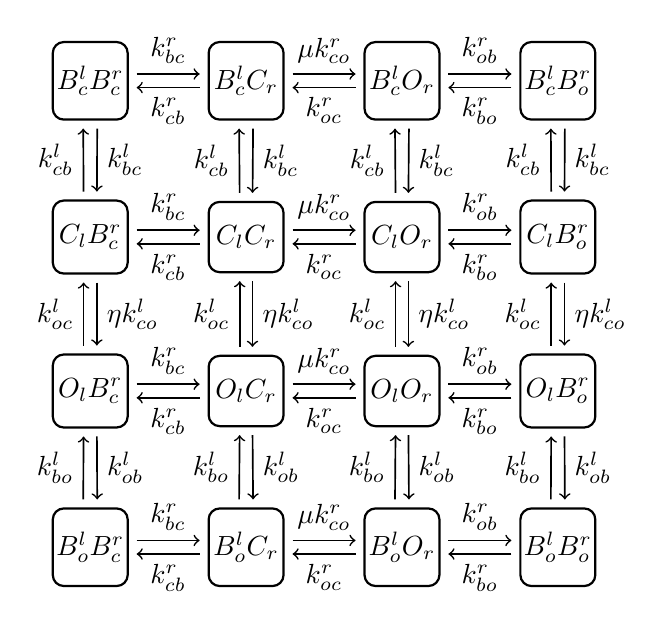
\begin{tikzpicture}[
   font=\sffamily,
   every matrix/.style={ampersand replacement=\&,column sep=1cm,row sep=1cm},
   state/.style={draw,thick,rounded corners,inner sep=.3cm},
   to/.style={->,semithick,shorten >=0.1cm,shorten <=0.1cm},
   Q/.style={->,semithick,sloped,pos=0.700000,shorten >=0.1cm,shorten <=0.1cm},
   every node/.style={auto}]
\matrix{
\node[state] (B_{c}^{l}B_{c}^{r}) {\parbox{10pt}{\centerline{$B_{c}^{l}B_{c}^{r}$}}};\&\node[state] (B_{c}^{l}C_{r}) {\parbox{10pt}{\centerline{$B_{c}^{l}C_{r}$}}};\&\node[state] (B_{c}^{l}O_{r}) {\parbox{10pt}{\centerline{$B_{c}^{l}O_{r}$}}};\&\node[state] (B_{c}^{l}B_{o}^{r}) {\parbox{10pt}{\centerline{$B_{c}^{l}B_{o}^{r}$}}};\\
\node[state] (C_{l}B_{c}^{r}) {\parbox{10pt}{\centerline{$C_{l}B_{c}^{r}$}}};\&\node[state] (C_{l}C_{r}) {\parbox{10pt}{\centerline{$C_{l}C_{r}$}}};\&\node[state] (C_{l}O_{r}) {\parbox{10pt}{\centerline{$C_{l}O_{r}$}}};\&\node[state] (C_{l}B_{o}^{r}) {\parbox{10pt}{\centerline{$C_{l}B_{o}^{r}$}}};\\
\node[state] (O_{l}B_{c}^{r}) {\parbox{10pt}{\centerline{$O_{l}B_{c}^{r}$}}};\&\node[state] (O_{l}C_{r}) {\parbox{10pt}{\centerline{$O_{l}C_{r}$}}};\&\node[state] (O_{l}O_{r}) {\parbox{10pt}{\centerline{$O_{l}O_{r}$}}};\&\node[state] (O_{l}B_{o}^{r}) {\parbox{10pt}{\centerline{$O_{l}B_{o}^{r}$}}};\\
\node[state] (B_{o}^{l}B_{c}^{r}) {\parbox{10pt}{\centerline{$B_{o}^{l}B_{c}^{r}$}}};\&\node[state] (B_{o}^{l}C_{r}) {\parbox{10pt}{\centerline{$B_{o}^{l}C_{r}$}}};\&\node[state] (B_{o}^{l}O_{r}) {\parbox{10pt}{\centerline{$B_{o}^{l}O_{r}$}}};\&\node[state] (B_{o}^{l}B_{o}^{r}) {\parbox{10pt}{\centerline{$B_{o}^{l}B_{o}^{r}$}}};\\
};
\draw[to]  (B_{c}^{l}B_{c}^{r}.10) to node {$k_{bc}^{r}$} (B_{c}^{l}C_{r}.170);
\draw[to]  (B_{c}^{l}B_{c}^{r}.280) to node {$k_{bc}^{l}$} (C_{l}B_{c}^{r}.80);
\draw[to]  (B_{c}^{l}C_{r}.190) to node {$k_{cb}^{r}$} (B_{c}^{l}B_{c}^{r}.350);
\draw[to]  (B_{c}^{l}C_{r}.10) to node {$\mu k_{co}^{r}$} (B_{c}^{l}O_{r}.170);
\draw[to]  (B_{c}^{l}C_{r}.280) to node {$k_{bc}^{l}$} (C_{l}C_{r}.80);
\draw[to]  (B_{c}^{l}O_{r}.190) to node {$k_{oc}^{r}$} (B_{c}^{l}C_{r}.350);
\draw[to]  (B_{c}^{l}O_{r}.10) to node {$k_{ob}^{r}$} (B_{c}^{l}B_{o}^{r}.170);
\draw[to]  (B_{c}^{l}O_{r}.280) to node {$k_{bc}^{l}$} (C_{l}O_{r}.80);
\draw[to]  (B_{c}^{l}B_{o}^{r}.190) to node {$k_{bo}^{r}$} (B_{c}^{l}O_{r}.350);
\draw[to]  (B_{c}^{l}B_{o}^{r}.280) to node {$k_{bc}^{l}$} (C_{l}B_{o}^{r}.80);
\draw[to]  (C_{l}B_{c}^{r}.100) to node {$k_{cb}^{l}$} (B_{c}^{l}B_{c}^{r}.260);
\draw[to]  (C_{l}B_{c}^{r}.10) to node {$k_{bc}^{r}$} (C_{l}C_{r}.170);
\draw[to]  (C_{l}B_{c}^{r}.280) to node {$\eta k_{co}^{l}$} (O_{l}B_{c}^{r}.80);
\draw[to]  (C_{l}C_{r}.100) to node {$k_{cb}^{l}$} (B_{c}^{l}C_{r}.260);
\draw[to]  (C_{l}C_{r}.190) to node {$k_{cb}^{r}$} (C_{l}B_{c}^{r}.350);
\draw[to]  (C_{l}C_{r}.10) to node {$\mu k_{co}^{r}$} (C_{l}O_{r}.170);
\draw[to]  (C_{l}C_{r}.280) to node {$\eta k_{co}^{l}$} (O_{l}C_{r}.80);
\draw[to]  (C_{l}O_{r}.100) to node {$k_{cb}^{l}$} (B_{c}^{l}O_{r}.260);
\draw[to]  (C_{l}O_{r}.190) to node {$k_{oc}^{r}$} (C_{l}C_{r}.350);
\draw[to]  (C_{l}O_{r}.10) to node {$k_{ob}^{r}$} (C_{l}B_{o}^{r}.170);
\draw[to]  (C_{l}O_{r}.280) to node {$\eta k_{co}^{l}$} (O_{l}O_{r}.80);
\draw[to]  (C_{l}B_{o}^{r}.100) to node {$k_{cb}^{l}$} (B_{c}^{l}B_{o}^{r}.260);
\draw[to]  (C_{l}B_{o}^{r}.190) to node {$k_{bo}^{r}$} (C_{l}O_{r}.350);
\draw[to]  (C_{l}B_{o}^{r}.280) to node {$\eta k_{co}^{l}$} (O_{l}B_{o}^{r}.80);
\draw[to]  (O_{l}B_{c}^{r}.100) to node {$k_{oc}^{l}$} (C_{l}B_{c}^{r}.260);
\draw[to]  (O_{l}B_{c}^{r}.10) to node {$k_{bc}^{r}$} (O_{l}C_{r}.170);
\draw[to]  (O_{l}B_{c}^{r}.280) to node {$k_{ob}^{l}$} (B_{o}^{l}B_{c}^{r}.80);
\draw[to]  (O_{l}C_{r}.100) to node {$k_{oc}^{l}$} (C_{l}C_{r}.260);
\draw[to]  (O_{l}C_{r}.190) to node {$k_{cb}^{r}$} (O_{l}B_{c}^{r}.350);
\draw[to]  (O_{l}C_{r}.10) to node {$\mu k_{co}^{r}$} (O_{l}O_{r}.170);
\draw[to]  (O_{l}C_{r}.280) to node {$k_{ob}^{l}$} (B_{o}^{l}C_{r}.80);
\draw[to]  (O_{l}O_{r}.100) to node {$k_{oc}^{l}$} (C_{l}O_{r}.260);
\draw[to]  (O_{l}O_{r}.190) to node {$k_{oc}^{r}$} (O_{l}C_{r}.350);
\draw[to]  (O_{l}O_{r}.10) to node {$k_{ob}^{r}$} (O_{l}B_{o}^{r}.170);
\draw[to]  (O_{l}O_{r}.280) to node {$k_{ob}^{l}$} (B_{o}^{l}O_{r}.80);
\draw[to]  (O_{l}B_{o}^{r}.100) to node {$k_{oc}^{l}$} (C_{l}B_{o}^{r}.260);
\draw[to]  (O_{l}B_{o}^{r}.190) to node {$k_{bo}^{r}$} (O_{l}O_{r}.350);
\draw[to]  (O_{l}B_{o}^{r}.280) to node {$k_{ob}^{l}$} (B_{o}^{l}B_{o}^{r}.80);
\draw[to]  (B_{o}^{l}B_{c}^{r}.100) to node {$k_{bo}^{l}$} (O_{l}B_{c}^{r}.260);
\draw[to]  (B_{o}^{l}B_{c}^{r}.10) to node {$k_{bc}^{r}$} (B_{o}^{l}C_{r}.170);
\draw[to]  (B_{o}^{l}C_{r}.100) to node {$k_{bo}^{l}$} (O_{l}C_{r}.260);
\draw[to]  (B_{o}^{l}C_{r}.190) to node {$k_{cb}^{r}$} (B_{o}^{l}B_{c}^{r}.350);
\draw[to]  (B_{o}^{l}C_{r}.10) to node {$\mu k_{co}^{r}$} (B_{o}^{l}O_{r}.170);
\draw[to]  (B_{o}^{l}O_{r}.100) to node {$k_{bo}^{l}$} (O_{l}O_{r}.260);
\draw[to]  (B_{o}^{l}O_{r}.190) to node {$k_{oc}^{r}$} (B_{o}^{l}C_{r}.350);
\draw[to]  (B_{o}^{l}O_{r}.10) to node {$k_{ob}^{r}$} (B_{o}^{l}B_{o}^{r}.170);
\draw[to]  (B_{o}^{l}B_{o}^{r}.100) to node {$k_{bo}^{l}$} (O_{l}B_{o}^{r}.260);
\draw[to]  (B_{o}^{l}B_{o}^{r}.190) to node {$k_{bo}^{r}$} (B_{o}^{l}O_{r}.350);
\end{tikzpicture}
\end{center}
\caption{The Markov model represented in Figure \ref{eq:m_rl} extended to
account for blockers for the LCC and the RyR.}
\label{Eq:m_rl2}
\end{figure}
This model consists of 16 separate states given by
\begin{equation}
\begin{tabular}
[c]{cccc}
$B_{c}^{l}B_{c}^{r}$ & $B_{c}^{l}C_{r}$ & $B_{c}^{l}O_{r}$ & $B_{c}^{l}B_{o}^{r}$\\
$C_{l}B_{c}^{r}$ & $C_{l}C_{r}$ & $C_{l}O_{r}$ & $C_{l}B_{o}^{r}$\\
$O_{l}B_{c}^{r}$ & $O_{l}C_{r}$ & $O_{l}O_{r}$ & $O_{l}B_{o}^{r}$\\
$B_{o}^{l} B_{c}^{r}$ & $B_{o}^{l}C_{r}$ & $B_{o}^{l}O_{r}$ &$B_{o}^{l}B_{o}^{r}$
\end{tabular}
\ \ \
\end{equation}
and the combined LCC and RyR drug is fully specified by
\begin{equation}
k_{cb}^{r},k_{bc}^{r},k_{bo}^{r},k_{ob}^{r},k_{cb}^{l},k_{bc}^{l}, k_{bo}^{l}, \text{ and }k_{ob}^{l}.
\end{equation}






\section[Probability density functions;16 state model]{Probability density functions associated with the 16-state model}

As mentioned in Chapter \ref{general} (see page \pageref{general}), it is convenient to use a more compact notation to represent the system of partial differential equations governing the probability density functions when the Markov model consists of numerous states. By using the notation introduced in Chapter \ref{general} , we can write the probability density system associated with the Markov model in Figure \ref{Eq:m_rl2} in the form
\begin{equation}
\frac{\partial\rho_{ij}}{\partial t}+\frac{\partial}{\partial x}\left(
a_{ij}^{x}\rho_{ij}\right)  +\frac{\partial}{\partial y}\left(  a_{ij}^{y}
\rho_{ij}\right)  =R_{ij}, \label{pdf16}
\end{equation}
where
\begin{align*}
R_{ij}  & =K_{i,j+1}^{i,j}\rho_{i,j+1}+K_{i+1,j}^{i,j}\rho_{i+1,j}
+K_{i,j-1}^{i,j}\rho_{i,j-1}+K_{i-1,j}^{i,j}\rho_{i-1,j}\\
& -\left(  K_{i,j}^{i,j+1}+K_{i,j}^{i+1,j}+K_{i,j}^{i,j-1}+K_{i,j}
^{i-1,j}\right)  \rho_{i,j}.
\end{align*}
 The flux terms are given by
\begin{align*}
a_{ij}^{x} &  =\gamma^{r}_{i}v_{r}\left(  y-x\right)  +v_{d}\left(
c_{0}-x\right) -\gamma^{l}_{j}J_{l} ,\\
a_{ij}^{y} &  =\gamma^{r}_{i}v_{r}\left(  x-y\right)  +v_{s}\left(
c_{1}-y\right)  ,
\end{align*}
where $\gamma^{r}_{i}=1$ when the RyR state is open and
$\gamma^{r}_{i}=0$ when the RyR state is closed and similarly for $\gamma^{l}$ and the LCC.

%Here we have formulated the system
%(\ref{Eq:m_rl2}) on the form (\ref{ninestates}) with an obvious extension from a nine state to
%a 16 state model. In the two dimensional numbering we
%have $\gamma_{ij}=\gamma^l_i \gamma^r_j$ where
%$\gamma^l_1=\gamma^l_3=\gamma^l_4=0$ and $\gamma^l_2=1$. And similarly,
%$\gamma^r_1=\gamma^r_2=\gamma^r_4=0$ and $\gamma^r_3=1$.

\section[RyR mutations]{RyR mutations under a varying transmembrane potential}

In this section, we assume that a mutation affects the RyR such that the
mutation severity index is increased. This problem has been discussed several times above, but here
we also need to take into account that the value of the transmembrane potential may change. In our computations, we use $\mu=3$ and
we try to repair the effect of the mutation by adding a closed state blocker
to the Markov model of the RyR channel.
The Markov model is shown in Figure \ref{m_ryr_c}.
\begin{figure}[ptb]
\begin{center}
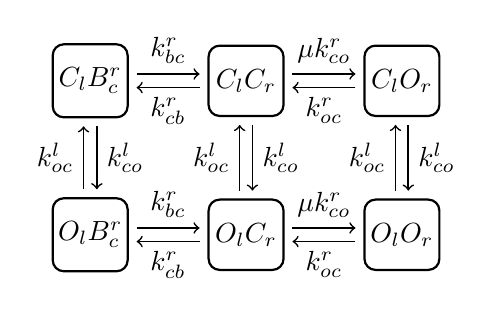
\begin{tikzpicture}[
   font=\sffamily,
   every matrix/.style={ampersand replacement=\&,column sep=1cm,row sep=1cm},
   state/.style={draw,thick,rounded corners,inner sep=.3cm},
   to/.style={->,semithick,shorten >=0.1cm,shorten <=0.1cm},
   Q/.style={->,semithick,sloped,pos=0.700000,shorten >=0.1cm,shorten <=0.1cm},
   every node/.style={auto}]
\matrix{
\node[state] (C_{l}B_{c}^{r}) {\parbox{10pt}{\centerline{$C_{l}B_{c}^{r}$}}};\&\node[state] (C_{l}C_{r}) {\parbox{10pt}{\centerline{$C_{l}C_{r}$}}};\&\node[state] (C_{l}O_{r}) {\parbox{10pt}{\centerline{$C_{l}O_{r}$}}};\\
\node[state] (O_{l}B_{c}^{r}) {\parbox{10pt}{\centerline{$O_{l}B_{c}^{r}$}}};\&\node[state] (O_{l}C_{r}) {\parbox{10pt}{\centerline{$O_{l}C_{r}$}}};\&\node[state] (O_{l}O_{r}) {\parbox{10pt}{\centerline{$O_{l}O_{r}$}}};\\
};
\draw[to]  (C_{l}B_{c}^{r}.10) to node {$k_{bc}^{r}$} (C_{l}C_{r}.170);
\draw[to]  (C_{l}B_{c}^{r}.280) to node {$k_{co}^{l}$} (O_{l}B_{c}^{r}.80);
\draw[to]  (C_{l}C_{r}.190) to node {$k_{cb}^{r}$} (C_{l}B_{c}^{r}.350);
\draw[to]  (C_{l}C_{r}.10) to node {$\mu k_{co}^{r}$} (C_{l}O_{r}.170);
\draw[to]  (C_{l}C_{r}.280) to node {$k_{co}^{l}$} (O_{l}C_{r}.80);
\draw[to]  (C_{l}O_{r}.190) to node {$k_{oc}^{r}$} (C_{l}C_{r}.350);
\draw[to]  (C_{l}O_{r}.280) to node {$k_{co}^{l}$} (O_{l}O_{r}.80);
\draw[to]  (O_{l}B_{c}^{r}.100) to node {$k_{oc}^{l}$} (C_{l}B_{c}^{r}.260);
\draw[to]  (O_{l}B_{c}^{r}.10) to node {$k_{bc}^{r}$} (O_{l}C_{r}.170);
\draw[to]  (O_{l}C_{r}.100) to node {$k_{oc}^{l}$} (C_{l}C_{r}.260);
\draw[to]  (O_{l}C_{r}.190) to node {$k_{cb}^{r}$} (O_{l}B_{c}^{r}.350);
\draw[to]  (O_{l}C_{r}.10) to node {$\mu k_{co}^{r}$} (O_{l}O_{r}.170);
\draw[to]  (O_{l}O_{r}.100) to node {$k_{oc}^{l}$} (C_{l}O_{r}.260);
\draw[to]  (O_{l}O_{r}.190) to node {$k_{oc}^{r}$} (O_{l}C_{r}.350);
\end{tikzpicture}
\end{center}
\caption{The Markov model represented in Figure \ref{eq:m_rl} extended to
include an RyR mutation and a closed state blocker for the RyR.}
\label{m_ryr_c}
\end{figure}

The closed state drug applied to the RyR channel is represented by the two
parameters $k_{cb}^{r}$ and $k_{bc}^{r}.$ We have seen above that for closed
state blockers of the RyR it is reasonable to define
\[
k_{cb}^{r}=\left(  \mu-1\right)  k_{bc}^{r},
\]
where the value of $k_{bc}^{r}$ remains to be decided.

\subsection{Theoretical closed state blocker repairs the open probabilities of the RyR CO-mutation}

Numerical results using the closed state drug shown in Figure \ref{m_ryr_c} are given
in Figure \ref{cicr:ryr_cbI}. Note that we aim to repair the probability of being in the open state and are not interested in whether the channel is in a blocked state or in a closed state. The probability of being in a closed or blocked state is therefore
added in the graphs. We observe from the graphs that
the mutant channel is completely repaired by the closed state blocker.

In Figure \ref{cicr:ryr_cbXY}, we show the development of the expected concentrations of the dyad ($x$) and the junctional sarcoplasmic reticulum  (JSR) ($y$) and observe that
the expected concentrations are repaired by a sufficiently strong version of the blocker associated with the closed state of the RyR channel.


FIGURE: [fig/cicr_ryr_cbI.pdf, width=500 frac=0.8] Total probabilities based on the model for the probability density functions associated with the Markov model
in Figure \ref{m_ryr_c}. A closed state blocker is applied, the mutation severity index is $\mu=3$, and the transmembrane potential is $V=0$ mV.
The plots show the total probability of being in the state OO, (OC+OB), CO, or (CC+CB) as a function of
$k^r_{bc}$. In the upper left plot, the total probability of being in the OO state is higher for the mutant than for the wild type. This is repaired by the closed
state drug. Similar results are shown for the other states.  label{cicr:ryr_cbI}FIGURE: [fig/cicr_ryr_cbXY.pdf, width=500 frac=0.8] Based on the probability density functions of the states OO, (OC+OB), CO, and (CC+CB), we can compute the
expected concentrations of the dyad ($x$) and the JSR ($y$). The wild type is denoted by $\circ$ and the RyR mutation index $\mu$ increases from one to three along the solid line. In the dashed line, we keep $\mu=3$ and increase the value of $k^r_{bc}$ from 0 $\rm{ms^{-1}}$ to 100 $\rm{ms^{-1}}$. We observe that as $k^r_{bc}$  increases, the
expected concentrations are completely repaired. The experiment is carried out for the case of $V=0$ mV. label{cicr:ryr_cbXY}
\subsection{The open state blocker does not work as well as the closed state blocker for CO-mutations in RyR}
%\K{zzz Kanskje denne underseksjonen heller burde st\r{a} under forrige seksjon
%siden den handler om RyR-mutasjoner?}
%\{I moved it}

In Table \ref{ryr_ob},  we report on the performance of the open and closed state blockers for the RyR mutation. Recall that the probability $\pi_{oo}$, the expected dyad concentration ($E^x_{oo}$), and the expected JSR concentration ($E^y_{oo}$) are defined on page \pageref{statistics}.  The closed blocker clearly is best suited to repair this mutation.





\begin{table}  \begin{center}
\begin{tabular}{|c|r|r|r|r|} \hline
&WT & MT & Optimal closed blocker & Optimal open blocker \\ \hline
$10^3\times\pi_{oo}$&2.75 & 5.11 & 2.74 & 0.81 \\ \hline
$E^x_{oo}$&51.87 & 45.62 & 51.92 & 52.46 \\ \hline
$E^y_{oo}$&751.76 & 544.30 & 751.99 & 713.89 \\ \hline
\end{tabular} \end{center}
\caption{Properties of the probability density function ($\rho_{oo}$) of being in the state OO with $\mu=3$ (and  $\eta=1$). The closed state blocker works fine in the sense that it is well suited for repairing a CO-mutation of the RyR.
The  open state blocker is unable to completely repair the effect of the mutation. The open state blocker is found using Matlab's {\it Fminsearch},
with a cost function defined to minimize the difference between the wild type and the mutation when the drug is applied.
In this table, WT and MT mean wild type and mutant, respectively, and  $V=0$ mV is used in the simulations.
%{\bf xxx Glenn:Something is wrong since the integral of $\rho_{oo}$ larger than one.}
%\G{These were scaled by 1000, now noted in the table.}
} \label{ryr_ob}
\end{table}



%{\bf: Glenn:} Can you make a plot of the type given in the upper left corner of Figure  \ref{cicr:ryr_cbXY}, Where you %have one panel for all the voltages:
%−80, −60, −40, −20, 0, 20 mV? We should comment on that this holds for varying voltage.

\section[LCC mutations]{LCC mutations under a varying transmembrane potential}

Next, we address the problem of defining a theoretical drug for LCC
mutations. We consider closed state LCC blockers of the form
given in Figure \ref{m_lcc_c} and open state blockers of the form
given in Figure \ref{m_lcc_o}.

\begin{figure}[ptb]
\begin{center}
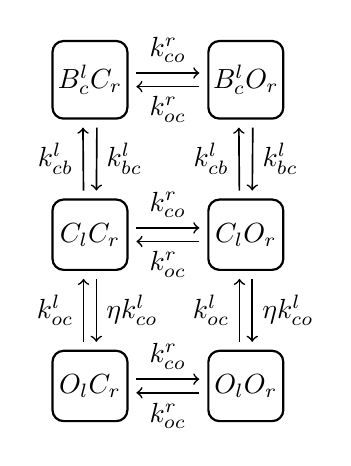
\begin{tikzpicture}[
   font=\sffamily,
   every matrix/.style={ampersand replacement=\&,column sep=1cm,row sep=1cm},
   state/.style={draw,thick,rounded corners,inner sep=.3cm},
   to/.style={->,semithick,shorten >=0.1cm,shorten <=0.1cm},
   Q/.style={->,semithick,sloped,pos=0.700000,shorten >=0.1cm,shorten <=0.1cm},
   every node/.style={auto}]
\matrix{
\node[state] (B_{c}^{l}C_{r}) {\parbox{10pt}{\centerline{$B_{c}^{l}C_{r}$}}};\&\node[state] (B_{c}^{l}O_{r}) {\parbox{10pt}{\centerline{$B_{c}^{l}O_{r}$}}};\\
\node[state] (C_{l}C_{r}) {\parbox{10pt}{\centerline{$C_{l}C_{r}$}}};\&\node[state] (C_{l}O_{r}) {\parbox{10pt}{\centerline{$C_{l}O_{r}$}}};\\
\node[state] (O_{l}C_{r}) {\parbox{10pt}{\centerline{$O_{l}C_{r}$}}};\&\node[state] (O_{l}O_{r}) {\parbox{10pt}{\centerline{$O_{l}O_{r}$}}};\\
};
\draw[to]  (B_{c}^{l}C_{r}.10) to node {$k_{co}^{r}$} (B_{c}^{l}O_{r}.170);
\draw[to]  (B_{c}^{l}C_{r}.280) to node {$k_{bc}^{l}$} (C_{l}C_{r}.80);
\draw[to]  (B_{c}^{l}O_{r}.190) to node {$k_{oc}^{r}$} (B_{c}^{l}C_{r}.350);
\draw[to]  (B_{c}^{l}O_{r}.280) to node {$k_{bc}^{l}$} (C_{l}O_{r}.80);
\draw[to]  (C_{l}C_{r}.100) to node {$k_{cb}^{l}$} (B_{c}^{l}C_{r}.260);
\draw[to]  (C_{l}C_{r}.10) to node {$k_{co}^{r}$} (C_{l}O_{r}.170);
\draw[to]  (C_{l}C_{r}.280) to node {$\eta k_{co}^{l}$} (O_{l}C_{r}.80);
\draw[to]  (C_{l}O_{r}.100) to node {$k_{cb}^{l}$} (B_{c}^{l}O_{r}.260);
\draw[to]  (C_{l}O_{r}.190) to node {$k_{oc}^{r}$} (C_{l}C_{r}.350);
\draw[to]  (C_{l}O_{r}.280) to node {$\eta k_{co}^{l}$} (O_{l}O_{r}.80);
\draw[to]  (O_{l}C_{r}.100) to node {$k_{oc}^{l}$} (C_{l}C_{r}.260);
\draw[to]  (O_{l}C_{r}.10) to node {$k_{co}^{r}$} (O_{l}O_{r}.170);
\draw[to]  (O_{l}O_{r}.100) to node {$k_{oc}^{l}$} (C_{l}O_{r}.260);
\draw[to]  (O_{l}O_{r}.190) to node {$k_{oc}^{r}$} (O_{l}C_{r}.350);
\end{tikzpicture}
\end{center}
\caption{The Markov model represented in Figure \ref{eq:m_rl} extended to
include an LCC mutation and a closed state blocker for the LCC.}
\label{m_lcc_c}
\end{figure}

\begin{figure}[ptb]
\begin{center}
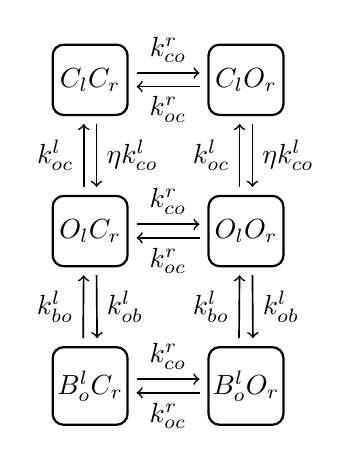
\begin{tikzpicture}[
   font=\sffamily,
   every matrix/.style={ampersand replacement=\&,column sep=1cm,row sep=1cm},
   state/.style={draw,thick,rounded corners,inner sep=.3cm},
   to/.style={->,semithick,shorten >=0.1cm,shorten <=0.1cm},
   Q/.style={->,semithick,sloped,pos=0.700000,shorten >=0.1cm,shorten <=0.1cm},
   every node/.style={auto}]
\matrix{
\node[state] (C_{l}C_{r}) {\parbox{10pt}{\centerline{$C_{l}C_{r}$}}};\&\node[state] (C_{l}O_{r}) {\parbox{10pt}{\centerline{$C_{l}O_{r}$}}};\\
\node[state] (O_{l}C_{r}) {\parbox{10pt}{\centerline{$O_{l}C_{r}$}}};\&\node[state] (O_{l}O_{r}) {\parbox{10pt}{\centerline{$O_{l}O_{r}$}}};\\
\node[state] (B_{o}^{l}C_{r}) {\parbox{10pt}{\centerline{$B_{o}^{l}C_{r}$}}};\&\node[state] (B_{o}^{l}O_{r}) {\parbox{10pt}{\centerline{$B_{o}^{l}O_{r}$}}};\\
};
\draw[to]  (C_{l}C_{r}.10) to node {$k_{co}^{r}$} (C_{l}O_{r}.170);
\draw[to]  (C_{l}C_{r}.280) to node {$\eta k_{co}^{l}$} (O_{l}C_{r}.80);
\draw[to]  (C_{l}O_{r}.190) to node {$k_{oc}^{r}$} (C_{l}C_{r}.350);
\draw[to]  (C_{l}O_{r}.280) to node {$\eta k_{co}^{l}$} (O_{l}O_{r}.80);
\draw[to]  (O_{l}C_{r}.100) to node {$k_{oc}^{l}$} (C_{l}C_{r}.260);
\draw[to]  (O_{l}C_{r}.10) to node {$k_{co}^{r}$} (O_{l}O_{r}.170);
\draw[to]  (O_{l}C_{r}.280) to node {$k_{ob}^{l}$} (B_{o}^{l}C_{r}.80);
\draw[to]  (O_{l}O_{r}.100) to node {$k_{oc}^{l}$} (C_{l}O_{r}.260);
\draw[to]  (O_{l}O_{r}.190) to node {$k_{oc}^{r}$} (O_{l}C_{r}.350);
\draw[to]  (O_{l}O_{r}.280) to node {$k_{ob}^{l}$} (B_{o}^{l}O_{r}.80);
\draw[to]  (B_{o}^{l}C_{r}.100) to node {$k_{bo}^{l}$} (O_{l}C_{r}.260);
\draw[to]  (B_{o}^{l}C_{r}.10) to node {$k_{co}^{r}$} (B_{o}^{l}O_{r}.170);
\draw[to]  (B_{o}^{l}O_{r}.100) to node {$k_{bo}^{l}$} (O_{l}O_{r}.260);
\draw[to]  (B_{o}^{l}O_{r}.190) to node {$k_{oc}^{r}$} (B_{o}^{l}C_{r}.350);
\end{tikzpicture}
\end{center}
\caption{The Markov model represented in Figure \ref{eq:m_rl} extended to
include an LCC mutation and an open state blocker for the LCC.}
\label{m_lcc_o}
\end{figure}

For the closed state blockers, we need to determine the two parameters
$k_{bc}^{l}$ and $k_{cb}^{l}$ and for the open state blockers we must determine
$k_{bo}^{l}$ and $k_{ob}^{l}.$ For the closed state blockers we define
\[
k_{cb}^{l}=\left(  \eta-1\right)  k_{bc}^{l}
\]
and we consider various values of $k_{bc}^{l}.$

%For the open state blocker we use (as above)
%straightforward optimization to minimize the norm xxx. This gives
%\[
%k_{ob}^{l}=xxx\text{ and }k_{bo}^{l}=xxx.
%\]

\subsection{The closed state blocker repairs the open probabilities of the LCC mutant}

The results of applying the theoretical closed state blocker associated with the closed state  (see Figure \ref{m_lcc_c}) of the LCC are given in Figures
\ref{cicr:lcc_cbI} to \ref{cicr:lcc_cb_V}. In the first figure, we show how the closed state blocker repairs the total probabilities and in the second figure we consider the expected concentrations. In Figure  \ref{cicr:lcc_cb_V}, we show how the expected concentrations are repaired for six values of the transmembrane potential.


FIGURE: [fig/cicr_lcc_cbI.pdf, width=500 frac=0.8] Total probabilities based on the model for the probability density functions associated with the Markov model
in Figure \ref{m_lcc_c}, where an LCC-type closed state blocker is included. The LCC mutation severity index is $\eta=3$ and the transmembrane potential is $V=0$ mV.
The plots show the total probability of being in the state OO, OC, (CO+BO), or (CC+BC) as a function of
$k^l_{bc}$. In the upper left plot, the total probability of being in the OO state is higher for the mutant than for the wild type. This is repaired by the closed state drug. Similar results are shown for the other states. label{cicr:lcc_cbI}FIGURE: [fig/cicr_lcc_cbXY.pdf, width=500 frac=0.8] Using the probability density functions of the states OO, OC, (CO+BO), and (CC+BC), we compute the
expected concentrations of the dyad ($x$) and the JSR ($y$). The wild type is denoted by $\circ$ and the LCC mutation index $\eta$ increases from one to three along the solid line. In the dashed line, we keep $\eta=3$ and increase the value of $k^l_{bc}$ from 0 $\rm{ms^{-1}}$ to 100 $\rm{ms^{-1}}$. We observe that as $k^l_{bc}$ increases, the
expected concentrations are completely repaired. The simulations are performed using $V=0$ mV. label{cicr:lcc_cbXY}FIGURE: [fig/cicr_lcc_cb_V.pdf, width=500 frac=0.8]  The expected  concentration of the dyad ($x$) and the JSR ($y$) for the OO state for the transmembrane potential
changing from -80 mV to 20 mV. The wild type is denoted by $\circ$ and the LCC mutation index $\eta$ increases from one to three along the solid line. In the dashed line, we keep $\eta=3$ and increase the value of $k^l_{bc}$ from 0 $\rm{ms^{-1}}$ to 100 $\rm{ms^{-1}}$.  In all cases, the closed state blocker repairs the effect of the mutation.
%{\bf xxx Glenn: check that text here is consistent with simulation. Remove if ok.}
 label{cicr:lcc_cb_V}%{\bf: Glenn:} Can you make a plot of the type given in the upper left corner of Figure  \ref{cicr:lcc_cbXY}, Where you have one panel for all the voltages:
%−80, −60, −40, −20, 0, 20 mV? We should comment on that this holds for varying voltage.

%\subsection{The closed state blocker for RyR does not repair the open probabilities of the LCC mutant}

%Here we check if it is possible to use a closed state blocker on RyR to repair the open probabilities of the LCC mutant. The last column of Table \ref{cross} shows the performanance in terms of restoring $\rho_{oo}$.

%\begin{table}  \begin{center}
%\begin{tabular}{|l|r|r|r|r|} \hline
%&WT & MT & $k^l_{cb}$ & $k^r_{cb}$ \\ \hline
%$\int \rho_{oo}$ &2.75 & 8.59 & 2.75 & 2.44 \\ \hline
%$\int x \rho_{oo}$&51.87 & 46.55 & 51.87 & 49.79 \\ \hline
%$\int y \rho_{oo}$ &751.76 & 580.88 & 751.77 & 657.87 \\ \hline
%\end{tabular} \end{center}
%\caption{Properties of $\rho_{oo}$, $\eta=3$ (and  $\mu=1$). Closed blocker on LCC works fine as seen before. Closed blocker on RyR not so much.The RyR blocker has been found using fminsearch. Cost function tried to minimize error in the overall expected values (overall meaning sum over all pdfs), mostly weighted on $x$ since this is the one that comunicates with the contractile units: $\sqrt{((x-x_{wt})/x_{wt})^2 + 0.1*((y-y_{wt})/y_{wt})^2}$
%} \label{cross}
%\end{table}



